\section{Commutativity of the Weak Queue Specification}
\label{wqueue}

To demonstrate how the strong queue interface, and the corresponding commutativity of transactions, prevents a scalable transactional queue implementation, we create a different queue operation interface---a \emph{weak queue specification}. This weak specification increases commutativity of operations and transactions, and \emph{does} allow for a scalable transactional queue implementation. This interface is shown in Figure~\ref{fig:wq_interface}, and differs from the strong queue specification because a pop operation returns a \texttt{future<bool>} instead of \texttt{bool}. A \texttt{future<bool>} has the property that the value of the future (a boolean) is only available after the operation completes (in a non-transactional setting), or after the containing transaction commits (in a transactional setting). This interface for pop does not change the behavior or guarantees of a non-transactional, strong queue pop described in Section~\ref{q_spec}.
 
In a transactional setting, however, these pop operations must satisfy both the invariants of a concurrent queue, as well as the invariant that, at commit time, two consecutive pops in the same transaction remove consecutive values off the queue (but perhaps not from the \emph{head} of the queue). Furthermore, the pop operations cannot pop the values that were pushed within the same transaction. The invariants for a push remain the same (two pushes in the same transaction must appear consecutively in the queue). 
The weak queue retains all the fairness properties of a concurrent queue: no value remains in the queue forever, because values are still removed in the order in which they are added. Like Schwarz~\cite{schwarz}, we see uses for the weak transactional queue as a buffer between producer and consumer activities, in which the exact ordering of values in the buffer is unimportant, and a transaction does not need to know exactly how many values were actually popped. Examples of valid weak queue transactional histories are shown in Table~\ref{tab:txnal_weakq_commute}.  

\begin{figure}[t]
    \centering
    \begin{lstlisting}
                        void push(const value_type& v); 
                        future<bool> pop();                     
    \end{lstlisting}
    \caption{Weak Queue Operations Interface}
    \label{fig:wq_interface}
\end{figure}

A weak transactional queue has greater commutativity than a strong transactional one. Individual pop operations within a transaction now commute with any operation, because they all return \texttt{future<bool>} when called. 
\texttt{COMMIT\_TXN} operations, however, now return a list of \texttt{bool} values (one for each pop operation within the transaction). 
Thus, instead of having to synchronize \emph{both} individual pop operations and \texttt{COMMIT\_TXN} operations of transactions (as the strong transactional queue must), the weak transactional queue only needs to synchronize the \texttt{COMMIT\_TXN} operations. This is because only \texttt{COMMIT\_TXN} operations have return values that can change based on the ordering of operations in the history, and only \texttt{COMMIT\_TXN} operations fail to commute. Informally, we can think of moving from the strong to the weak queue specification as condensing all individual strong pop operations into one operation: the \texttt{COMMIT\_TXN} operation. The non-commutativity of all individual strong pop operations is now ``contained'' by the \texttt{COMMIT\_TXN} operation.\footnote{Again, we can consider adding front operations to create front-pop operations (a pop operation immediately preceded by a front operation). A weak front-pop returns a future representing the contents of the front and the return value of the pop, which is instantiated at commit time. Given this specification, all weak front-pops commute (because they all return futures), but \texttt{COMMIT\_TXN} operations fail to commute in precisely those scenarios in which strong front-pops fail to commute. Thus, moving from the strong queue specification to the weak queue specification is equivalent to condensing of all strong front-pop operations into one operation, the \texttt{COMMIT\_TXN} operation.}

We claim that synchronizing these \texttt{COMMIT\_TXN} operations is no more difficult than synchronizing strong queue pops in a non-transactional setting. We use the same commutativity reasoning we used to reason about commutativity between individual strong pops and pushes to reason about commutativity between weak \texttt{COMMIT\_TXN} operations. A weak \texttt{COMMIT\_TXN} operation can be described as a pair of a pop-group operation and a push-group operation: in order to satisfy our specification, all pops of the transaction need to be installed together at commit time, and all pushes of the transaction need to be installed together at commit time. It is clear that a pop-group that encounters an empty queue will not commute with another pop-group or another a push-group; thus, we see that a pop-group has equivalent commutativity behavior to a strong pop, and a push-group has equivalent commutativity behavior to a strong push. Indeed, performing a weak \texttt{COMMIT\_TXN} operation, like performing a strong pop operation, requires protected access to the queue's head, and does not scale.

To further support our point, we implement a weak transactional flat combining queue, and demonstrate that flat combining's synchronization mechanism for a strong, non-transactional pop can be used by this weak transactional queue with minimal modifications.

\begin{table}[H]
    \centering
    \singlespace
    \begin{tabular}{|l|l|}
        \hline
\multicolumn{1}{|c|}{Valid History Interleaving} & \multicolumn{1}{c|}{Serialized Forms of History}\\
        \hline
\begin{lstlisting}
// Q empty
(T1, START_TXN, ())                       
(T2, START_TXN, ())                       
(T2, Q.pop(), ())                       
(T1, Q.pop(), ())                       
(T1, Q.push(a), ())                       
(T1, Q.push(a), ())                       
(T1, COMMIT_TXN, {false})                       
(T2, COMMIT_TXN, {true/false})                       
\end{lstlisting} &
\begin{lstlisting}
// Q empty
(T1, START_TXN, ())                       
(T1, Q.pop(), ())                       
(T1, Q.push(a), ())                       
(T1, Q.push(a), ())                       
(T1, COMMIT_TXN, {false})                       
(T2, START_TXN, ())                       
(T2, Q.pop(), ())                       
(T2, COMMIT_TXN, {true})                       
 ------------------------------
// Q empty
(T2, START_TXN, ())                       
(T2, Q.pop(), ())                       
(T2, COMMIT_TXN, {false})                       
(T1, START_TXN, ())                       
(T1, Q.pop(), ())                       
(T1, Q.push(a), ())                       
(T1, Q.push(a), ())                       
(T1, COMMIT_TXN, {false})                       
\end{lstlisting}\\
\hline
\begin{lstlisting}
// Q empty
(T1, START_TXN, ())                       
(T2, START_TXN, ())                       
(T1, Q.push(a), ())                       
(T1, Q.pop(), ())                       
(T1, Q.pop(), ())                       
(T2, Q.pop(), ())                       
(T1, Q.push(a), ())                       
(T1, COMMIT_TXN, {false, false})                       
(T2, COMMIT_TXN, {true/false})                       
\end{lstlisting} &
\begin{lstlisting}
// Q empty
(T1, START_TXN, ())                       
(T1, Q.push(a), ())                       
(T1, Q.pop(), ())                       
(T1, Q.pop(), ())                       
(T1, Q.push(a), ())                       
(T1, COMMIT_TXN, {false, false})                       
(T2, START_TXN, ())                       
(T2, Q.pop(), ())                       
(T2, COMMIT_TXN, {true})                       
 ------------------------------
// Q empty
(T2, START_TXN, ())                       
(T2, Q.pop(), ())                       
(T2, COMMIT_TXN, {false})                       
(T1, START_TXN, ())                       
(T1, Q.push(a), ())                       
(T1, Q.pop(), ())                       
(T1, Q.pop(), ())                       
(T1, Q.push(a), ())                       
(T1, COMMIT_TXN, {true, false})                       
\end{lstlisting}\\
    \hline
    
    \end{tabular}
    \caption[Examples of valid weak queue transaction histories.]{Examples of valid weak queue transaction histories. The history interleavings shown on the left are valid regardless of whether $T2$ returns \texttt{true} or \texttt{false}, because we can find a serialized form of the history in either case.}
    \label{tab:txnal_weakq_commute}
    \end{table}

\subsection{The Weak Transactional Flat Combining Queue}
The Weak Transactional Flat Combining Queue (WT-FCQueue) demonstrates how the flat combining technique's performance depends upon the commutativity of operations of a particular queue specification, and how this commutativity changes in a transactional setting. It also supports our claim that the commutativity in a weak transactional queue is equivalent to the commutativity in a strong non-transactional queue.

WT-FCQueue implements the weak transactional queue specification using \emph{futures}: instead of returning \texttt{bool}, a pop will return a future. The future will be instantiated with a \texttt{true} or \texttt{false} boolean value at commit time, but prior to that time, the future's value cannot be accessed.
At commit time, our implementation performs a pop using the non-transactional flat combining \texttt{<POP>} request, and assigns the corresponding boolean return value to the corresponding future. All pushes from the transaction are also installed at commit time using the \texttt{<PUSH, write\_list>} request described earlier. We note that both pop and push requests do not need to access the queue during execution time. This allows us to minimize the number of flat combining calls: we do not need to generate additional flat combining calls during transaction execution because the queue does not need to be accessed until commit time.

Our implementation satisfies a weaker specification than the weak queue specification described above: in our implementation, pops are not guaranteed to be consecutive. However, we hypothesize that a queue that installs all pops at once---by posting, at commit time, a \texttt{<POP, num\_pops>} request that returns a list of booleans---will perform no worse than our current method of pops (or may perhaps even perform better). This is because the synchronization is still restricted to the point at which the \texttt{COMMIT\_TXN} operations occur in the history, and in both our actual and proposed implementations, only a single thread can access the queue at this point.

\subsection{Evaluation and Results}

\begin{figure}[t]
    \centering
    {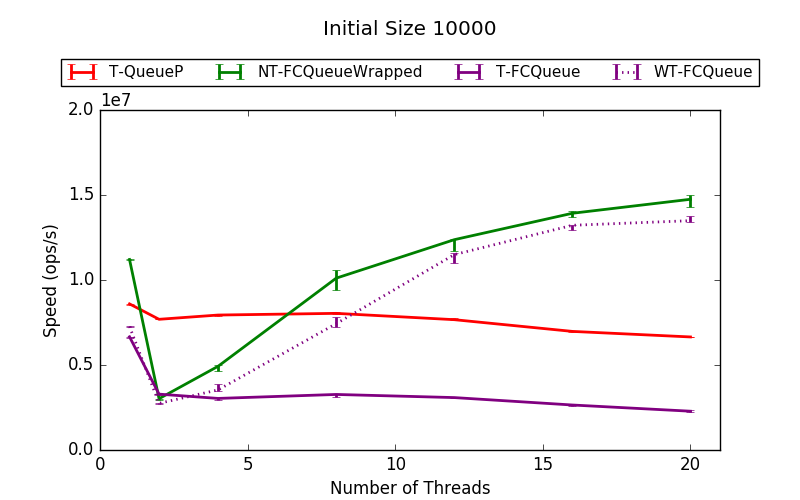
\includegraphics[width=\textwidth]{fcqueues/lpQ:RandSingleOps10000.png}}
    \caption{WT-FCQueue Performance: Multi-Thread Singletons Test}
    \label{fig:wtqs}
\end{figure}

We evaluate the weak transactional flat-combining queue on the same benchmarks described in Section~\ref{q_microbenchmarks} to compare against the strong transactional flat-combining queue (T-FCQueue), T-QueueP, and NT-FCQueueWrapped. Selected results are shown in Figure~\ref{fig:wtqs}.

While WT-FCQueue does not perform as well as its non-transactional counterpart, NT-FCQueue, the performance of WT-FCQueue exceeds that of T-QueueO, T-QueueP, and T-FCQueue, which all provide transactional guarantees under the strong queue specification. We see gains in performance over T-QueueP up to 1.5$\times$ as the number of threads accessing the queue increases to 20; the WT-FCQueue begins to outperform T-QueueP as the number of threads increases past 7. The WT-FCQueue outperforms T-FCQueue starting at 4 threads and achieves performance up to about 5$\times$ by 20 threads.
 
The WT-FCQueue does not experience any aborts. This is because the weak transactional flat combining algorithm never needs to prevent other threads' requests from being performed by the combiner thread. Because of the lack of aborts, the WT-FCQueue significantly outperforms T-FCQueue; this demonstrates the effectiveness of the flat combining technique in the weak transactional setting. 

Our results show significant improvements in the performance of the flat combining algorithm when satisfying the weak transactional queue specification, compared to its performance when satisfying the strong transactional specification. This demonstrates that the choice of queue specification, and therefore the commutativity of queue operations, directly affects the effectiveness of the flat combining algorithm in a transactional setting. We argue that the modifications to provide transactional guarantees with our strong queue specification critically impair the performance of the flat combining algorithm, and that these modifications cannot be avoided. Thus, scalable performance of a strong flat combining queue is unlikely to be achievable in a transactional setting.
